\end{multicols}
\section{Results}
In our optimization of the model we iterated over the hyperparemeters in the order: No. of layers, learning rate, debth of layers and kernel size. For each hyperparameter we adjusted the value and allowed the multi-task model to train for 10 epochs and then evaluate accuracy of both the Q8 secondary structure prediction as well as the relative and absolute solvent accessibiliy on both the validation and test set.\\
In choosing which values to continue with for the final model we only considered results on the validation set, and attempted to balance accuracy with model size and trainability.\\
Once we had found what configurations performed the best on the respective parameters, we trained both our single- and multi-task models with these parameters for 20 epochs and compared the results.

\subsection{Hyperparameters}
\subsubsection{No. of layers}
Variying the number of layers in the model greatly affects the size of the model and thus also the time taken to train it. Further, adding more layers increases the risk of overfitting (factcheck lige det...).\\
In our tests we evaluated from two to five hidden layers. Note, that the output layer is not counted in this number.

% Please add the following required packages to your document preamble:
% \usepackage[normalem]{ulem}
% \useunder{\uline}{\ul}{}
\begin{table}[H]
\centering
\begin{tabular}{lcccccc}
\multicolumn{7}{c}{\textbf{No. of layers}} \\
\multicolumn{7}{c}{\textit{Layer debth = 80, kernel size = 11, learning rate = 0.00025, batch size = 4}} \\ \hline
\multicolumn{1}{l|}{} & \multicolumn{3}{c|}{{\ul Validation set}} & \multicolumn{3}{c}{{\ul Test set}} \\
\multicolumn{1}{c|}{Layers} & Q8 & \begin{tabular}[c]{@{}c@{}}Relative\\ solvent\\ accessibility\end{tabular} & \multicolumn{1}{c|}{\begin{tabular}[c]{@{}c@{}}Absolute\\ solvent\\ accessibility\end{tabular}} & Q8 & \begin{tabular}[c]{@{}c@{}}Relative\\ solvent\\ accessibility\end{tabular} & \begin{tabular}[c]{@{}c@{}}Absolute\\ solvent\\ accessibility\end{tabular} \\ \hline
\multicolumn{1}{l|}{2} & 69.79\% & 81.94\% & \multicolumn{1}{c|}{80.58\%} & 69.783\% & 82.001\% & 80.413\% \\
\multicolumn{1}{l|}{3} & 70.08\% & 82.69\% & \multicolumn{1}{c|}{81.10\%} & 70.447\% & 82.259\% & 80.701\% \\
\multicolumn{1}{l|}{4} & 70.11\% & 82.90\% & \multicolumn{1}{c|}{81.18\%} & 70.143\% & 82.291\% & 80.528\% \\
\multicolumn{1}{l|}{5} & 69.48\% & 82.73\% & \multicolumn{1}{c|}{81.13\%} & 69.343\% & 82.158\% & 80.365\% \\
\multicolumn{1}{l|}{16} & 68.15\% & 82.15\% & \multicolumn{1}{c|}{80.42\%} & 68.459\% & 81.595\% & 79.924\% \\
\multicolumn{1}{l|}{32} & 66.94\% & 81.61\% & \multicolumn{1}{c|}{79.85\%} & 67.279\% & 81.196\% & 79.483\% \\
\multicolumn{1}{l|}{64} & 65.10\% & 80.97\% & \multicolumn{1}{c|}{79.25\%} & 65.100\% & 80.644\% & 78.899\%
\end{tabular}
\end{table}
\noindent We made the dicision after this test to continue with 3 hidden layers, as we did not feel that the gained accuracy by advancing to 4 matched the increased cost of training the network.


\subsubsection{Learning rate}
Having a bad learning rate puts the model in risk of several things. A learning rate too small will possibly trap the model in a local minimum, whereas a learning rate too big will risk not being able to hit global maxima, but constantly shifting around them. Further, a lower learning rate means more time needed to train, while a larger learning rate might in the worst case actually miss a global maximum.\\
Below are the results of our tests of learning rate.
% Please add the following required packages to your document preamble:
% \usepackage[normalem]{ulem}
% \useunder{\uline}{\ul}{}
\begin{table}[H]
\centering
\begin{tabular}{lcccccc}
\multicolumn{7}{c}{\textbf{Learning rate}} \\
\multicolumn{7}{c}{\textit{Layer debth = 80, kernel size = 11, 3 hidden layers, batch size = 4}} \\ \hline
\multicolumn{1}{l|}{} & \multicolumn{3}{c|}{{\ul Validation set}} & \multicolumn{3}{c}{{\ul Test set}} \\
\multicolumn{1}{c|}{\begin{tabular}[c]{@{}c@{}}Learning\\ rate\end{tabular}} & Q8 & \begin{tabular}[c]{@{}c@{}}Relative\\ solvent\\ accessibility\end{tabular} & \multicolumn{1}{c|}{\begin{tabular}[c]{@{}c@{}}Absolute\\ solvent\\ accessibility\end{tabular}} & Q8 & \begin{tabular}[c]{@{}c@{}}Relative\\ solvent\\ accessibility\end{tabular} & \begin{tabular}[c]{@{}c@{}}Absolute\\ solvent\\ accessibility\end{tabular} \\ \hline
\multicolumn{1}{l|}{0.00005} & 66.85\% & 81.61\% & \multicolumn{1}{c|}{79.89\%} & 66.958\% & 81.052\% & 79.490\% \\
\multicolumn{1}{l|}{0.0001} & 68.71\% & 82.18\% & \multicolumn{1}{c|}{80.42\%} & 68.983\% & 81.737\% & 80.042\% \\
\multicolumn{1}{l|}{0.00025} & 70.38\% & 82.78\% & \multicolumn{1}{c|}{81.23\%} & 70.386\% & 82.077\% & 80.576\% \\
\multicolumn{1}{l|}{0.0005} & 70.83\% & 82.86\% & \multicolumn{1}{c|}{81.13\%} & 70.624\% & 82.136\% & 80.437\% \\
\multicolumn{1}{l|}{0.001} & 70.66\% & 82.75\% & \multicolumn{1}{c|}{80.92\%} & 70.287\% & 82.040\% & 80.426\% \\
\multicolumn{1}{l|}{0.0025} & 69.12\% & 81.67\% & \multicolumn{1}{c|}{79.59\%} & 68.590\% & 81.294\% & 79.806\%
\end{tabular}
\end{table}
\noindent Not only did the non-optimal learning rates not perform as well as 0.0005, but they also trained significantly slower, as seen on the graph below.
\begin{figure}[H]
  \centering
  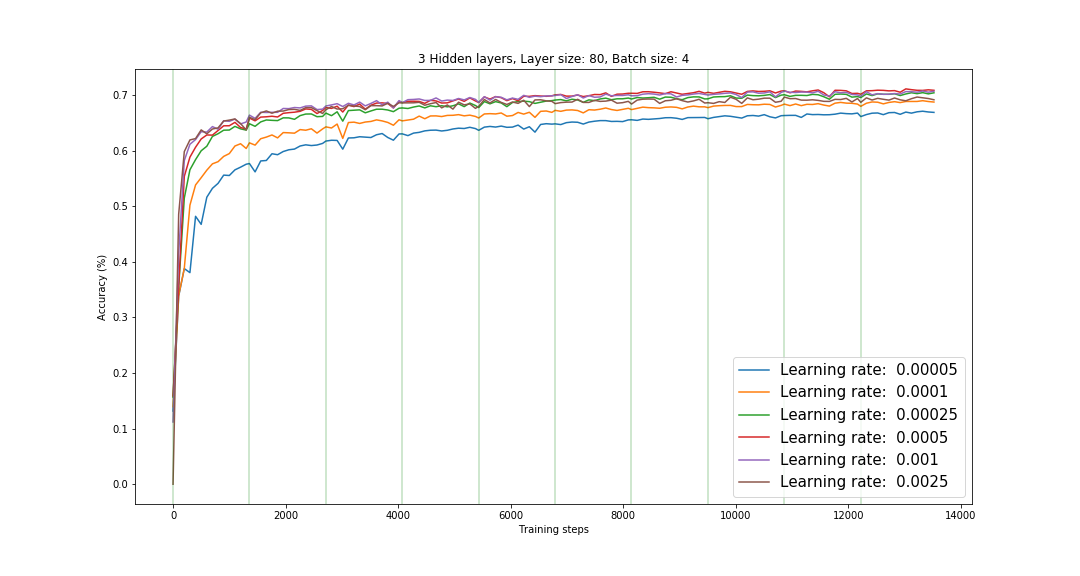
\includegraphics[width=\linewidth]{../graphs/new/learning_rate}
  \caption{Accuracy on the validation with varying learning rate. The green lines represent epochs.}
\end{figure}
For the remainder of the tests we used a learning rate of 0.0005.

\subsubsection{Depth of layers}
As with the number of layers, the depth affects both model potential complex predictive performance and model weight and size. We started from the depth of 100 as also used by Xi et al. and found that no increase in performance was acheived by adding more depth, however some gains were made by shallowing down the layers a bit.

\begin{table}[H]
\centering
\begin{tabular}{lcccccc}
\multicolumn{7}{c}{\textbf{Layer depth}} \\
\multicolumn{7}{c}{\textit{Learning rate = 0.0005, kernel size = 11, 3 hidden layers, batch size = 4}} \\ \hline
\multicolumn{1}{l|}{} & \multicolumn{3}{c|}{{\ul Validation set}} & \multicolumn{3}{c}{{\ul Test set}} \\
\multicolumn{1}{c|}{Depth} & Q8 & \begin{tabular}[c]{@{}c@{}}Relative\\ solvent\\ accessibility\end{tabular} & \multicolumn{1}{c|}{\begin{tabular}[c]{@{}c@{}}Absolute\\ solvent\\ accessibility\end{tabular}} & Q8 & \begin{tabular}[c]{@{}c@{}}Relative\\ solvent\\ accessibility\end{tabular} & \begin{tabular}[c]{@{}c@{}}Absolute\\ solvent\\ accessibility\end{tabular} \\ \hline
\multicolumn{1}{l|}{50} & 70.14\% & 81.94\% & \multicolumn{1}{c|}{81.07\%} & 70.436\% & 82.280\% & 80.395\% \\
\multicolumn{1}{l|}{60} & 70.77\% & 82.68\% & \multicolumn{1}{c|}{81.17\%} & 70.407\% & 81.931\% & 80.295\% \\
\multicolumn{1}{l|}{70} & 70.03\% & 82.97\% & \multicolumn{1}{c|}{81.20\%} & 70.931\% & 82.392\% & 80.723\% \\
\multicolumn{1}{l|}{80} & 70.86\% & 82.78\% & \multicolumn{1}{c|}{81.14\%} & 70.881\% & 82.228\% & 80.535\% \\
\multicolumn{1}{l|}{90} & 71.19\% & 83.09\% & \multicolumn{1}{c|}{81.37\%} & 70.973\% & 82.472\% & 80.734\% \\
\multicolumn{1}{l|}{100} & 70.95\% & 82.05\% & \multicolumn{1}{c|}{80.31\%} & 71.007\% & 82.704\% & 80.602\%
\end{tabular}
\end{table}
\noindent As is seen in the table a depth of 90 filters proved most accurate on our tests. Below is shown a graph of three of the values, illustrating how a depth of 90 performed better than the two other continuously throughout training. Refer to the appendix for at graph containing all the tested  depths.
\begin{figure}[H]
  \centering
  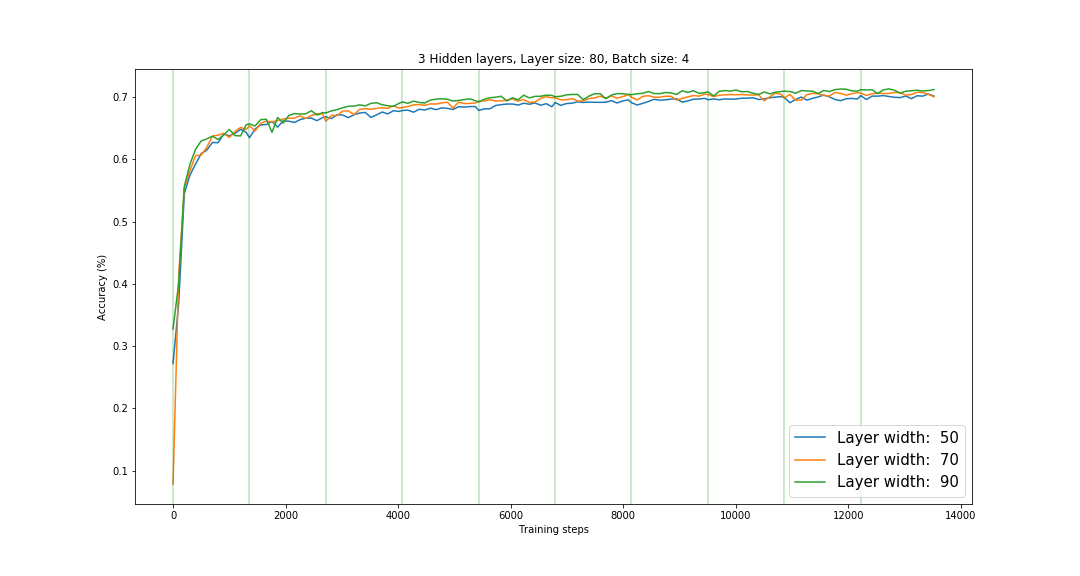
\includegraphics[width=\linewidth]{../graphs/new/layer_width_1}
  \caption{Accuracy on the validation set with varying layer depth.}
\end{figure}
\subsubsection{Kernel size}
In the article by Xi et al, a kernel size of 11 was chosen on the basis that the average length of an $\alpha$-helix chain, and in accordance with this we tested values in the vicinity. For the sake of padding we stuck to uneven values.\\
While the first tests fokus on keeping the same size of kernel throughout the layers in the model, we also performed a series of tests using increasing, decreasing, pyramid-shaped and valley-shaped progressions of kernel sizes.

% Please add the following required packages to your document preamble:
% \usepackage[normalem]{ulem}
% \useunder{\uline}{\ul}{}
\begin{table}[H]
\centering
\begin{tabular}{ccccccc}
\multicolumn{7}{c}{\textbf{Kernel sizes}} \\
\multicolumn{7}{c}{\textit{Learning rate = 0.0005, layer depth = 90, 3 hidden layers, batch size = 4}} \\ \hline
\multicolumn{1}{l|}{} & \multicolumn{3}{c|}{{\ul Validation set}} & \multicolumn{3}{c}{{\ul Test set}} \\
\multicolumn{1}{c|}{\begin{tabular}[c]{@{}c@{}}Kernel\\ Size\end{tabular}} & Q8 & \begin{tabular}[c]{@{}c@{}}Relative\\ solvent\\ accessibility\end{tabular} & \multicolumn{1}{c|}{\begin{tabular}[c]{@{}c@{}}Absolute\\ solvent\\ accessibility\end{tabular}} & Q8 & \begin{tabular}[c]{@{}c@{}}Relative\\ solvent\\ accessibility\end{tabular} & \begin{tabular}[c]{@{}c@{}}Absolute\\ solvent\\ accessibility\end{tabular} \\ \hline
\multicolumn{1}{c|}{5} & 71.00\% & 82.54\% & \multicolumn{1}{c|}{81.20\%} & 70.455\% & 82.405\% & 80.657\% \\
\multicolumn{1}{c|}{7} & 71.50\% & 82.24\% & \multicolumn{1}{c|}{81.00\%} & 71.616\% & 82.241\% & 80.611\% \\
\multicolumn{1}{c|}{9} & 71.44\% & 82.95\% & \multicolumn{1}{c|}{81.24\%} & 71.409\% & 82.363\% & 80.714\% \\
\multicolumn{1}{c|}{11} & 70.94\% & 82.15\% & \multicolumn{1}{c|}{80.52\%} & 70.957\% & 82.592\% & 80.742\% \\
\multicolumn{1}{c|}{13} & 70.82\% & 82.49\% & \multicolumn{1}{c|}{80.97\%} & 70.903\% & 82.389\% & 80.605\% \\ \hline
\multicolumn{1}{c|}{{[}5,7,9,11{]}} & 71.55\% & 82.98\% & \multicolumn{1}{c|}{81.48\%} & 71.636\% & 82.525\% & 80.963\% \\
\multicolumn{1}{c|}{{[}7,9,11,13{]}} & 71.17\% & 82.75\% & \multicolumn{1}{c|}{81.20\%} & 71.284\% & 82.778\% & 80.856\% \\
\multicolumn{1}{c|}{{[}11,9,7,5{]}} & 71.21\% & 82.43\% & \multicolumn{1}{c|}{81.00\%} & 71.387\% & 82.221\% & 80.712\% \\
\multicolumn{1}{c|}{{[}7,9,9,7{]}} & 70.78\% & 82.88\% & \multicolumn{1}{c|}{81.34\%} & 71.588\% & 82.673\% & 80.956\% \\
\multicolumn{1}{c|}{{[}9,7,7,9{]}} & 71.20\% & 82.87\% & \multicolumn{1}{c|}{81.26\%} & 71.424\% & 82.365\% & 80.845\%
\end{tabular}
\end{table}
\begin{figure}[H]
  \centering
  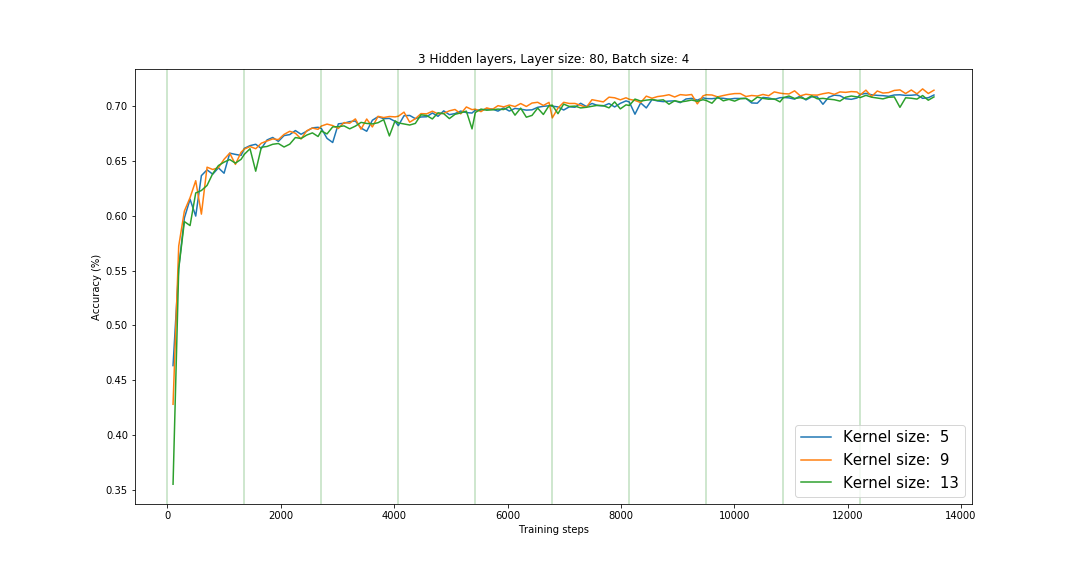
\includegraphics[width=\linewidth]{../graphs/new/kernel_sizes_2}
  \caption{Constant kernel size.}
\end{figure}

\begin{figure}[H]
  \centering
  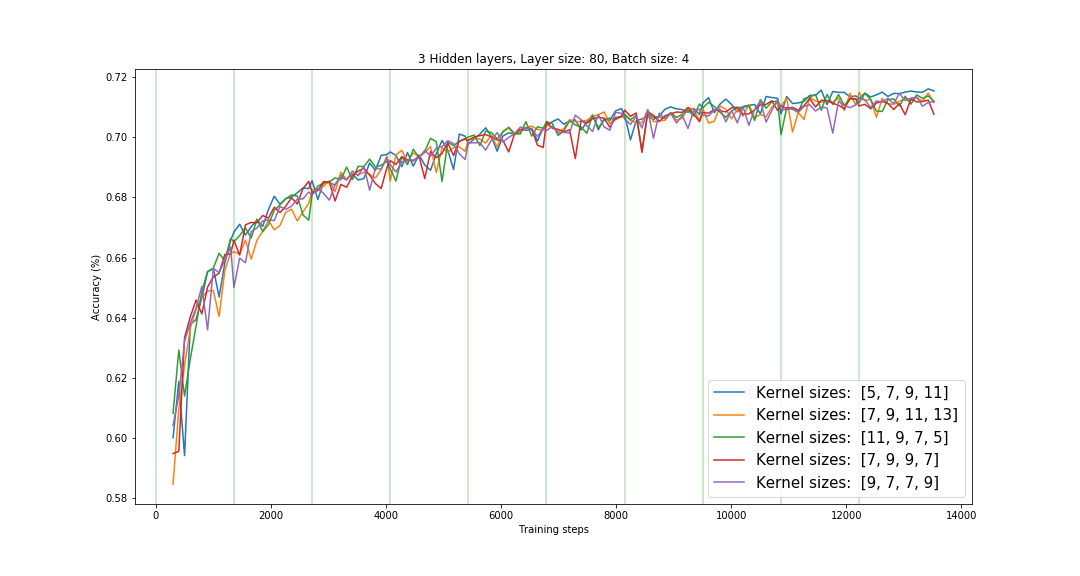
\includegraphics[width=\linewidth]{../graphs/new/kernel_sizes_1}
  \caption{Varying kernel size.}
\end{figure}

\noindent As with the layer depth, not all values are shown in the graph - refer to the appendix for a graph with all values.\\
It became clear that using a progressively rising size of kernels a significant increase was seen in accuracy. For the final model we opted to use kernel sizes [5, 7, 9, 11].\\
What is interesting about the data shown above, is that while one would expect larger kernel sizes to increase performance, or at the very least not decrease it (since the model should learn just to 'ignore' extra space in the kernel), the model's performance did indeed decrease as the kernel sizes grew.



\subsection{Final predictive capabilities}
Having performed the series of tests described above we settled on the following architecture:
\begin{table}[H]
\centering
\begin{tabular}{lr}
\multicolumn{2}{c}{\textbf{Final model architecture}} \\ \hline
\multicolumn{1}{l|}{\textit{Hyperparameter}} & \textit{Value} \\ \hline
\multicolumn{1}{l|}{No. of hidden layers} & 3 \\
\multicolumn{1}{l|}{Learning rate} & 0.0005 \\
\multicolumn{1}{l|}{Layer depth} & 90 \\
\multicolumn{1}{l|}{Kernel sizes} & {[}5, 7, 9, 11{]}
\end{tabular}
\end{table}

\noindent Implementing this with PyTorch gave us the following evaluation of the model:
\begin{lstlisting}
CNN(
  (conv1): Sequential(
    (0): Conv1d(44, 90, kernel_size=(5,), stride=(1,), padding=(3,))
    (1): ReLU()
  )
  (conv2): Sequential(
    (0): Conv1d(90, 90, kernel_size=(7,), stride=(1,), padding=(4,))
    (1): ReLU()
  )
  (conv3): Sequential(
    (0): Conv1d(90, 90, kernel_size=(9,), stride=(1,), padding=(5,))
    (1): ReLU()
  )
  (out): Sequential(
    (0): Conv1d(90, 11, kernel_size=(11,), stride=(1,), padding=(6,))
  )
)
\end{lstlisting}
\noindent Note that the architecture for the three models was essentially the same, however differed in implementation by the way the data was split in the end, the activation functions and the loss functions, not shown in the evaluation above but explained earlier in this paper.\\
\\
We then allowed the three models to train on the data set for 20 epochs each, monitoring how they performed on the validation and test during this time. It became clear that all of the models began to overfit to the training set at some point during this training, so we also recorded when the model was at its best for comparison purposes.

\subsubsection{Solvent accessibility}
In the case of relative solvent accessibility the multi-task learning model performed almost identically to the single-task model, while the single-task slightly outperformed the multitask model in regards to the absolute solvent accessibility.

\begin{table}[h]
\centering
\begin{tabular}{lclcl}
 & \multicolumn{4}{c}{\textbf{Relative Solvent Accessibility}} \\
 & \multicolumn{2}{c|}{\textit{Validation}} & \multicolumn{2}{c}{\textit{Test}} \\ \cline{2-5} 
 & \multicolumn{1}{l}{Epoch} & \multicolumn{1}{l|}{Accuracy} & \multicolumn{1}{l}{Epoch} & Accuracy \\
Single-task & 13 & \multicolumn{1}{l|}{83.245\%} & 11 & 82.752\% \\
Multi-task & 15 & \multicolumn{1}{l|}{83.263\%} & 12 & 82.763\%
\end{tabular}
\end{table}

\begin{figure}[H]
  \centering
  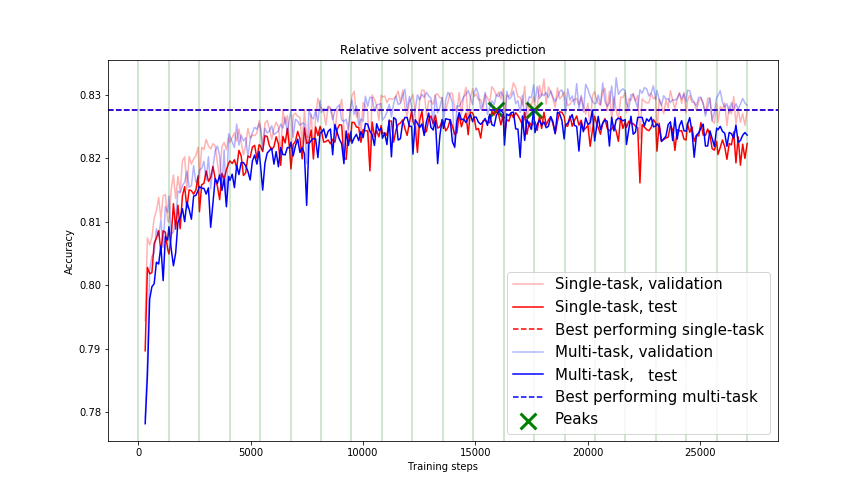
\includegraphics[width=\linewidth]{../graphs/final/rel_final_small}
  \caption{Peak performance on the relative solvent accessibility. Green lines represent epochs.}
\end{figure}

\begin{table}[h]
\centering
\begin{tabular}{lclcl}
 & \multicolumn{4}{c}{\textbf{Absolute Solvent Accessibility}} \\
 & \multicolumn{2}{c|}{\textit{Validation}} & \multicolumn{2}{c}{\textit{Test}} \\ \cline{2-5} 
 & \multicolumn{1}{l}{Epoch} & \multicolumn{1}{l|}{Accuracy} & \multicolumn{1}{l}{Epoch} & Accuracy \\
Single-task & 12 & \multicolumn{1}{l|}{81.671\%} & 11 & 81.006\% \\
Multi-task & 11 & \multicolumn{1}{l|}{81.636\%} & 10 & 80.912\%
\end{tabular}
\end{table}

\begin{figure}[H]
  \centering
  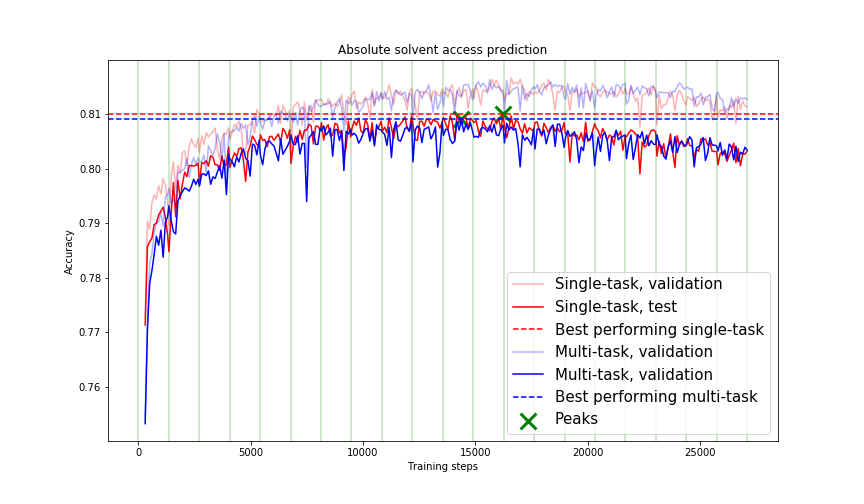
\includegraphics[width=\linewidth]{../graphs/final/abs_final_small}
  \caption{Peak performance on the absolute solvent accessibility.}
\end{figure}

\noindent It becomes clear that the the decisions made about the parameters throughout our process were indeed made on the basis of optimizing the accuracy on the validation set. Further, the results here seem to indicate that there are noteworthy differences between the test and validation sets.\\
As is also the case for predicting the secondary structures, the effects of overfitting are seen quite clearly. In most of the runs the models reach their predictive ceiling already around 12 or 13 epochs, before losing accuracy on the test and validations sets again as the model starts overfitting to the training set.
%\begin{table}[]
%\centering
%\begin{tabular}{lclll}
%\multicolumn{1}{c}{\textbf{}} & \multicolumn{4}{c}{\textbf{Solvent Accessibility}} \\
% & \multicolumn{2}{c}{{\ul Single-task}} & \multicolumn{2}{c}{{\ul Multi-task}} \\
% & Epoch & \multicolumn{1}{c}{Accuracy} & \multicolumn{1}{c}{Epoch} & \multicolumn{1}{c}{Accuracy} \\ \cline{2-5} 
%\multicolumn{1}{l|}{Feature} & \multicolumn{4}{c|}{\textit{Validation set}} \\
%\multicolumn{1}{l|}{Relative} & \multicolumn{1}{l}{13} & \multicolumn{1}{l|}{83.245\%} & 15 & \multicolumn{1}{l|}%{83.263\%} \\
%\multicolumn{1}{l|}{Absolute} & \multicolumn{1}{l}{12} & \multicolumn{1}{l|}{81.671\%} & 11 & \multicolumn{1}{l|}%{81.636\%} \\ \cline{2-5} 
%\multicolumn{1}{l|}{} & \multicolumn{4}{c|}{\textit{Test set}} \\
%\multicolumn{1}{l|}{Relative} & \multicolumn{1}{l}{11} & \multicolumn{1}{l|}{82.752\%} & 12 & \multicolumn{1}{l|}%{82.763\%} \\
%\multicolumn{1}{l|}{Absolute} & \multicolumn{1}{l}{11} & \multicolumn{1}{l|}{81.006\%} & 10 & \multicolumn{1}{l|}%{80.912\%}
%\end{tabular}
%\end{table}

\subsubsection{Secondary Structures}
By implementing multi-task learning in the model we saw a slight increase in the accuracy when predicting protein secondary structures as compared to the single-task model. We did however observe that while the two models both moved towards predictive ceilings not that far apart, the multi-task model reached it significantly faster.
\begin{table}[h]
\centering
\begin{tabular}{lclcl}
 & \multicolumn{4}{c}{\textbf{Q8 Secondary Structures}} \\
 & \multicolumn{2}{c|}{\textit{Validation}} & \multicolumn{2}{c}{\textit{Test}} \\ \cline{2-5} 
 & \multicolumn{1}{l}{Epoch} & \multicolumn{1}{l|}{Accuracy} & \multicolumn{1}{l}{Epoch} & Accuracy \\
Single-task & 17 & \multicolumn{1}{l|}{71.410\%} & 19 & 71.239\% \\
Multi-task & 12 & \multicolumn{1}{l|}{71.558\%} & 11 & 71.566\%
\end{tabular}
\end{table}

\begin{figure}[H]
  \centering
  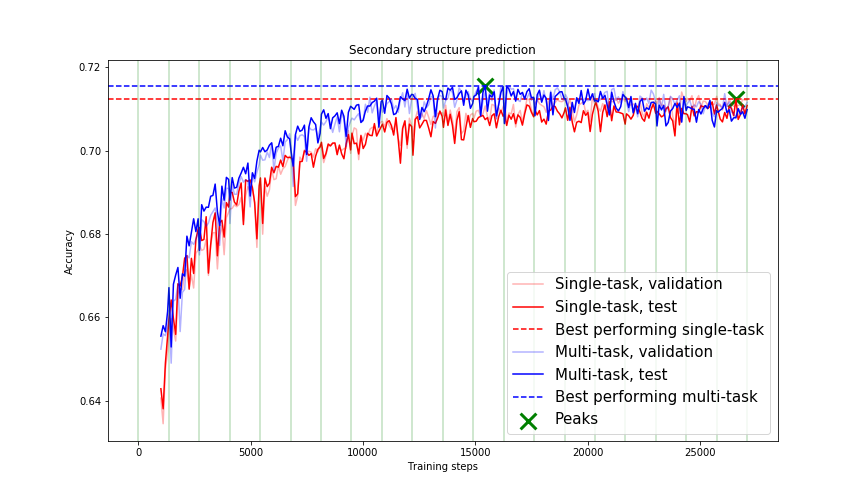
\includegraphics[width=\linewidth]{../graphs/final/final_secondary_small}
  \caption{Peak performance on the absolute solvent accessibility.}
\end{figure}

\noindent Again the effects of overfitting to the training data set is seen, however not to the same extent as was the case for the solvency features. \\
One can observe that although the optimal accuracy for the two models did not differ enormously in the end, the multi-task learning model consistently performed better than the single-task during the majority of the training session.

%\newpage
\begin{multicols}{2}





















